\hypertarget{part-1-design-2}{%
\section{Part 1, design 2}\label{part-1-design-2}}

\centering
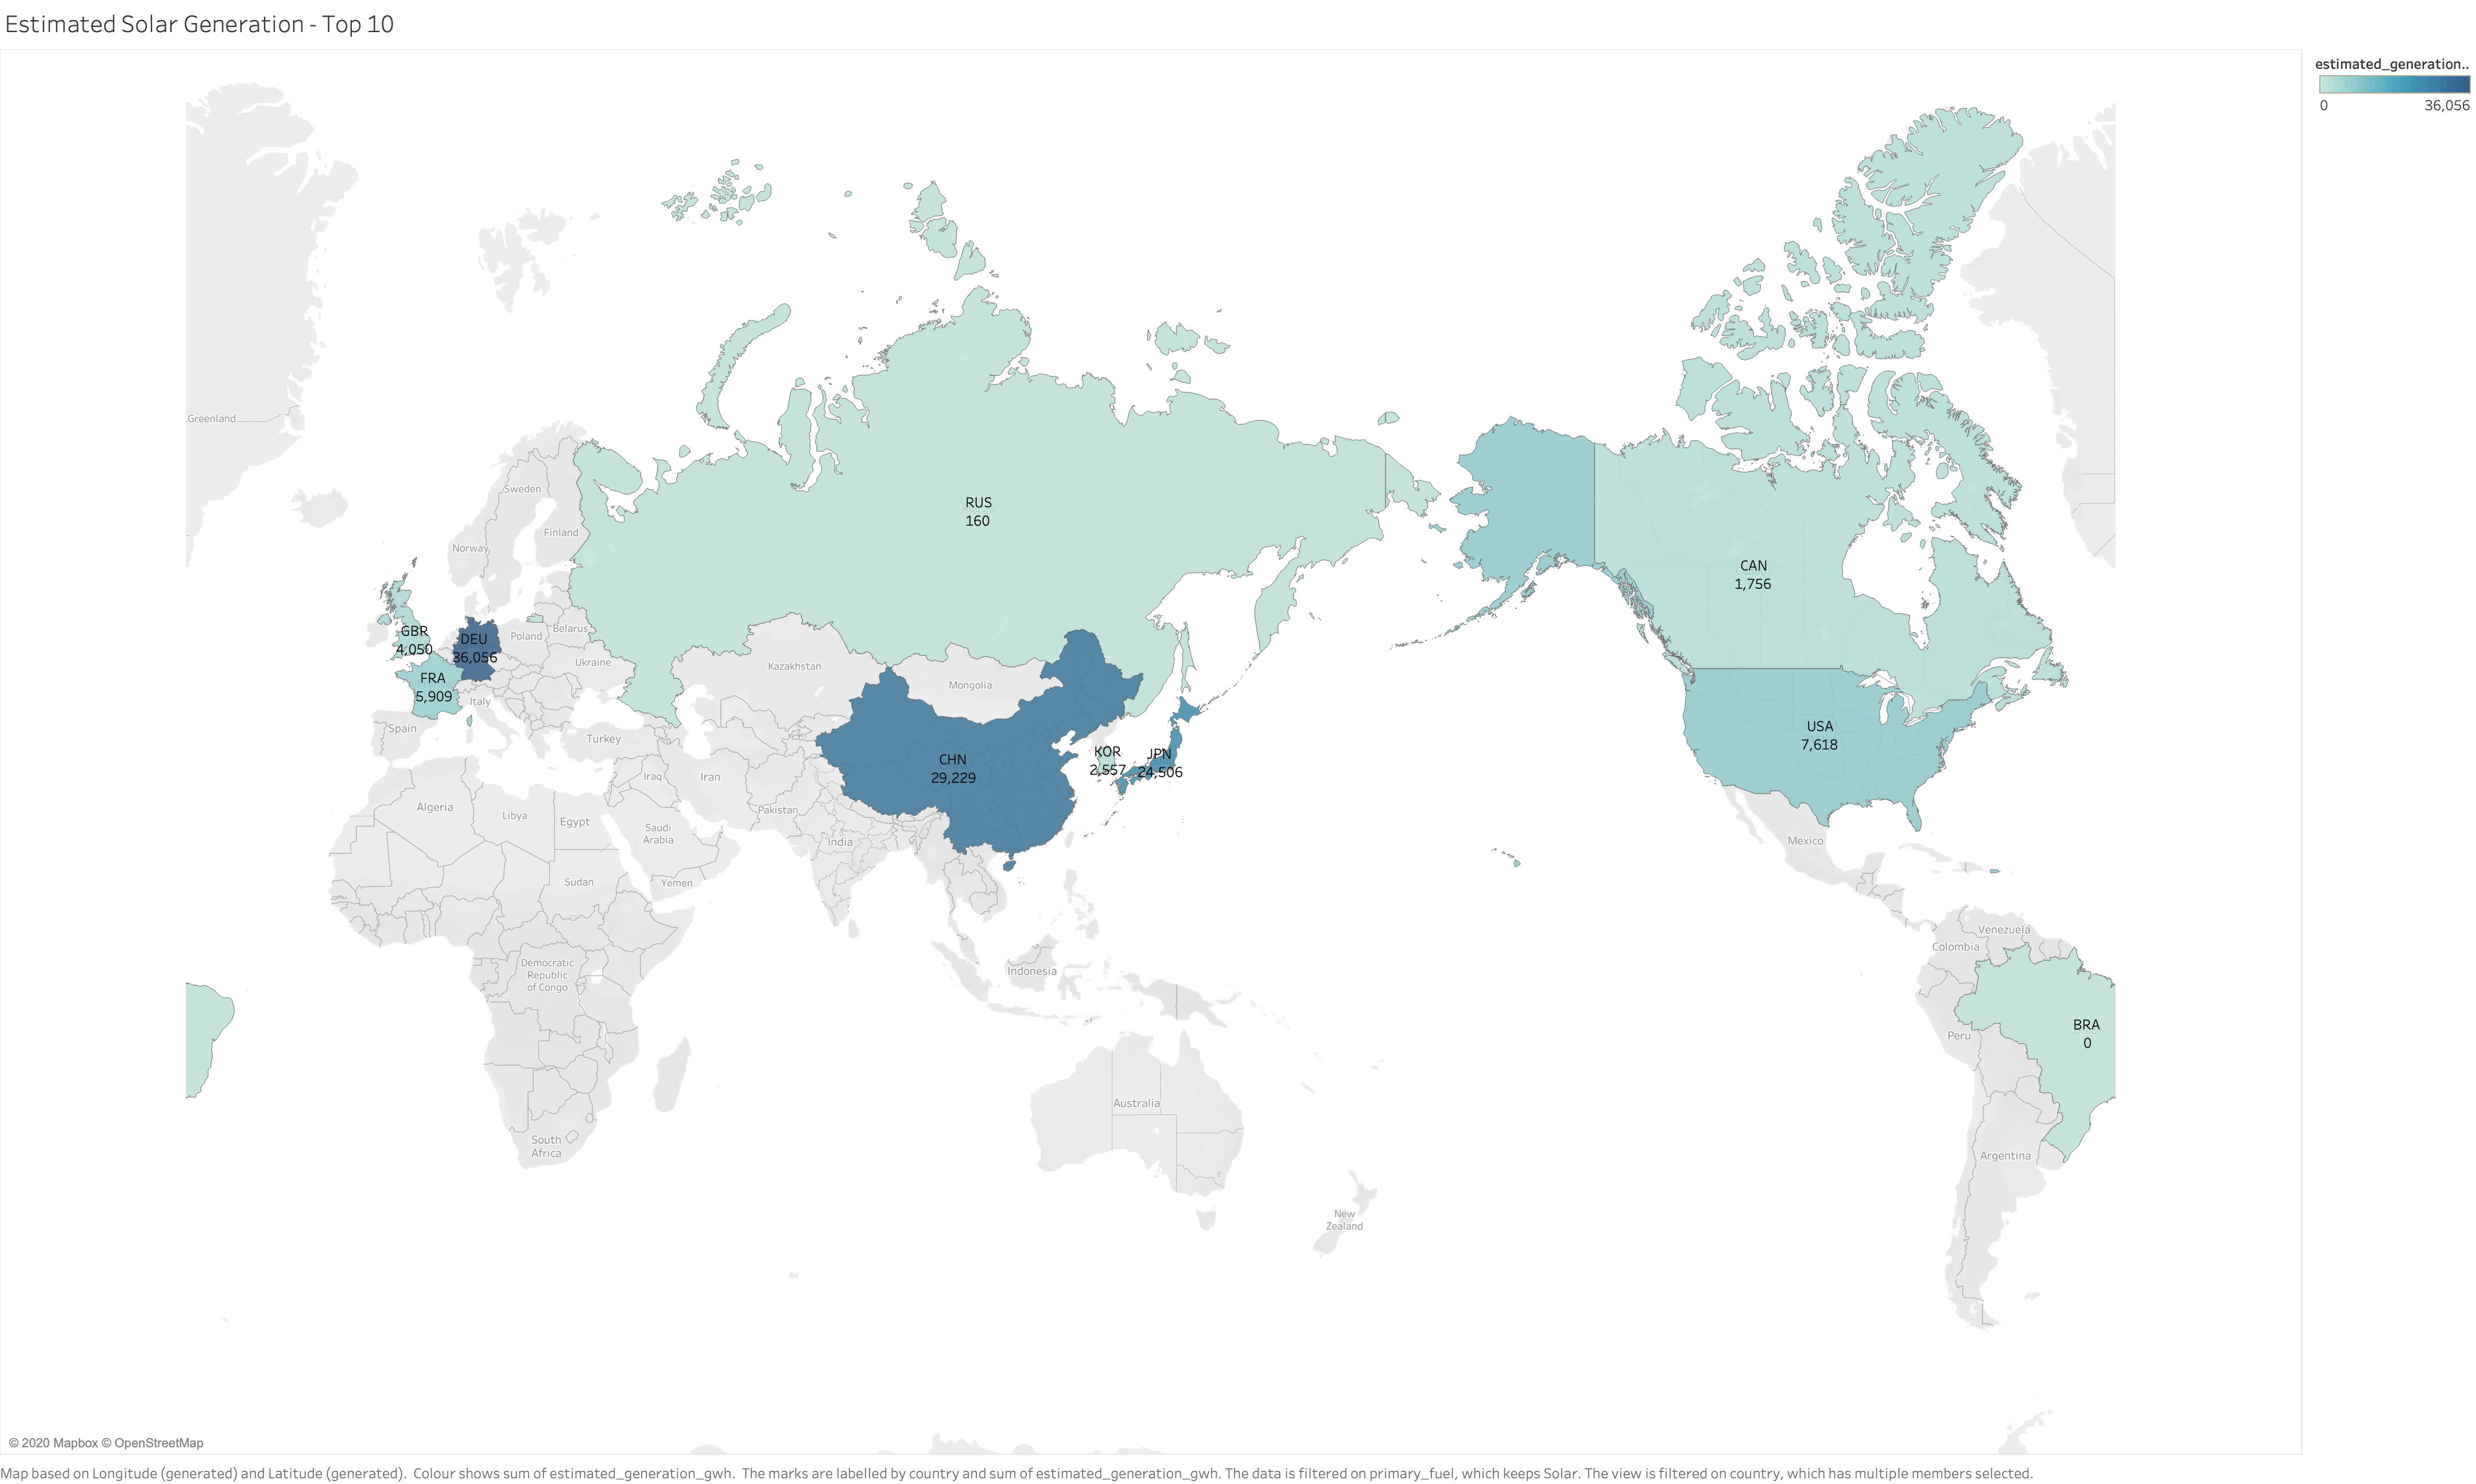
\includegraphics[width=15cm]{Viz2.png}

\hypertarget{description}{%
\subsubsection{Description}\label{description}}

\begin{description}
\item[Visual Design Type:]
Map
\item[Name of Tool:]
Tableua
\item[Country:]
France, Germany, Great Britain, Russia, China, Japan, South Korea, USA, Canada, Brazil.
\item[Year:]
2018
\item[Visual Mappings:]
\begin{itemize}
	\tightlist
	\item[  ]
\end{itemize}
\begin{itemize}
\tightlist
\item
  \textbf{mapping 1}: X and Y axis use the longitude and latitude values, this produces the map.
\end{itemize}

\begin{itemize}
\tightlist
\item
  \textbf{mapping 2}: Country is used to label the visualisation as well as the text. Colour is used to give a scale of the values, with dark being the biggest and a lighter colour being the smallest.
\end{itemize}
\item[Unique Observation:]
Germany is estimated to have the highest amount of solar energy created in 2018, at a value of 36,056. China is the second biggest estimation of solar power generated.

Weirdly enough, most counties around the equator are not in the top 10 of solar power energy generated. Brazil being the only one. You would think that this would be an effective source to tap into.

\item[Data Preparation:] Two filters have been applied, primary fuel, which is set to solar and country, which just shows the top 10 based on the sum of the estimated generation of energy.
\end{description}  